%%%%%%%%%%%%%%%%%%%%%%%%%%%%%%%%%%%%%%%%%%%%%%%%%%%%%%%%%%%%%%%%%%%%%%%%%%%%%%%
%
% 
% 
%%%%%%%%%%%%%%%%%%%%%%%%%%%%%%%%%%%%%%%%%%%%%%%%%%%%%%%%%%%%%%%%%%%%%%%%%%%%%%%


\chapter{Simulation Method}
\label{sec:Simulation Method}

\section{FEM}
The finite element method (FEM) is a numerical technique for solving problems which are described by partial differential equations or can be formulated as functional minimization. A domain of interest is is divided into an assembly of finite elements. Approximating functions in finite elements are determined
in terms of nodal values of a physical field which is sought. A continuous physical problem is transformed into a discretized finite element problem with unknown nodal values. For a linear problem a system of linear algebraic equations should be solved. Values inside finite elements can be recovered
using nodal values. FEM then uses variational methods from the calculus of variations to approximate a solution by minimizing an associated error function.
Two features of the FEM are worth to be mentioned:
\begin{itemize}
\item Piece-wise approximation of physical fields on finite elements provides good precision even with
simple approximating functions (increasing the number of elements we can achieve any precision).
\item Locality of approximation leads to sparse equation systems for a discretized problem. This helps to
solve problems with very large number of nodal unknowns.
\end{itemize}

\subsection{Steps in FEM}
Finite Element Method can be generalized into these steps.
\begin{itemize}
 
 \item The physical problem has to be defined. All the desired results and the geometry of the problem have to be specified.

\item The mathematical model has to be formulated.
The physical problem has to be formulated as an (initial) boundary value problem, e.g. by means of partial differential equations with boundary and, if required, initial conditions.

\item The FE model has to be setup, which means that the mathematical model has to be discretised and the equations are solved. The structure is subdivided into finite elements, the solution is approximated element-wise and computed at the nodes of these elements. By this procedure, the differential equations are transferred into a system of algebraic equations

\begin{equation}
K.u = F
\end{equation}
For a static stress analysis, the unknown nodal values subsumed in u are the nodal displacements, K is the stiffness matrix and f contains the nodal forces. This system of equations has to be solved for the unknown nodal values

\begin{equation}
u = K^{-1}.f
\end{equation}

Subsequently, the dependent variables have to be computed in a so-called post-processing step. For a stress analysis the strains, the stresses, equivalent stresses and further variables are derived from the nodal displacement values and are usually displayed graphically.

\item The FE model yields a numerical solution which is an approximation of the exact solution of the mathematical problem. It has to be verified that the numerical solution is accurate enough and, if not, the FE model has to be improved. A more accurate solution can be obtained by choosing a larger number of nodes, which results in smaller finite elements. This, however, leads to higher computational effort such that an FE solution always represents a reasonable compromise between accuracy and computational effort.


\item When a satisfying numerical solution is found, the results have to be interpreted and validated. This is usually done by comparing them to those obtained from experiments. If the numerical solution does not sufficiently capture the relevant phenomena, the physical problem or the mathematical model might have to be adapted. The comparison between numerical and experimental results can also be used to e.g. identify material parameters.
\end{itemize}



\subsection{Constitutive Laws}

Elastic Modulus and Poisson's Ratio In 1D Stress State
The one-dimensional Hooke’s law relates 1D normal stress to 1D extensional strain through two material parameters the modulus of elasticity $E$, also called Young's modulus and Poisson's ratio $\nu$. The modulus of elasticity connects axial stress $\sigma$ to axial strain $\epsilon$:
\begin{equation}
\sigma = E\epsilon \label{Hooke's law}
\end{equation}

Poisson's ratio $\nu$ is defined as ratio of lateral strain to axial strain:
\begin{equation}
\nu = \abs{\frac{lateral strain}{axial strain}} = -\frac{lateral strain}{axial strain}
\end{equation}
The $-$ sign is introduced for convenience so that $\nu$ comes out positive. For structural materials $\nu$ lies in the range $0.0 \leq \nu <0.5$. For most metals $\nu \approx 0.25$–$0.35$. For concrete and ceramics, $\nu \approx 0.10$. For cork $\nu \approx 0$. For rubber, $\nu \approx 0.5$ to 3 places. A material for which $\nu = 0.5$ is called incompressible.

\subsubsection{Shear Modulus In 1D Stress State}

The shear modulus $G$ connects a shear strain $\gamma$ to the corresponding shear stress $\tau$:
\begin{equation}
\tau = G\gamma \label{Bulk modulus}
\end{equation} 

"Corresponding" means that if $\gamma$ = $\gamma_{xy}$, say, then $\tau = \tau_{xy}$, and similarly for the other shear components. The shear modulus is usually obtained from a torsion test. It turns out that the 3 material properties $E$, $\tau$ and $G$ for an elastic isotropic material are not independent, but are connected by the relations
\begin{equation}
G = \frac{E}{2(1 + \nu)} \label{isotropic}
\end{equation}
which means that if two of them are known by measurement, the third one can be obtained from the relations \ref{isotropic}. In practice the three properties are often measured independently, and the (approximate) verification of \ref{isotropic} gives an idea of how isotropic the material is.


\subsubsection{Shear Modulus In 3D Stress State}

\begin{figure}[h]
\centering
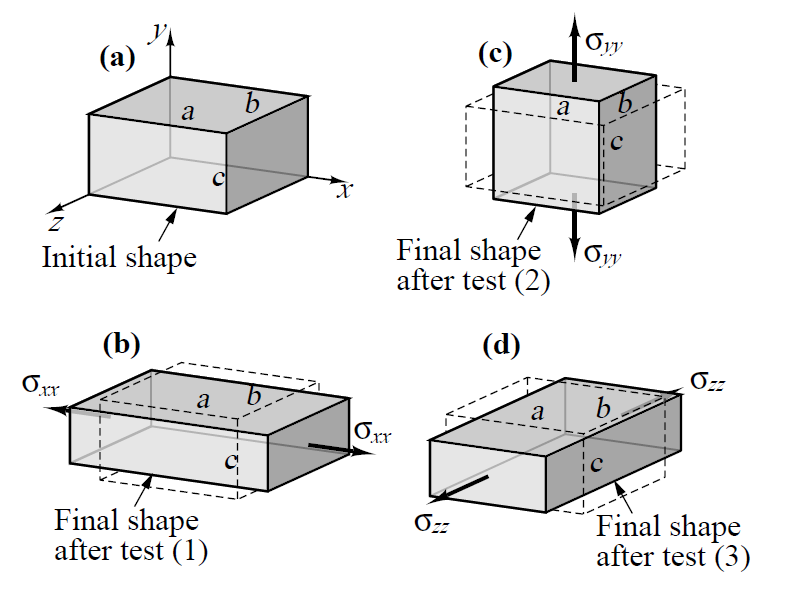
\includegraphics[scale=0.4]{../images/hookes.png}
\caption{Three tension tests are assumed to be carried out along $x, y, z$, respectively, and strains superposed.}
\label{fig:hookes}
\end{figure}


We now generalize the foregoing equations to the three-dimensional case, still assuming that the
material is elastic and isotropic. Consider a cube of material aligned with the axes ${x, y, z}$, as
shown in figure \ref{fig:hookes}. Imagine that three tension tests, labeled (1), (2) and (3) respectively, are
conducted along $x, y$ and $z$, respectively. Pulling the material by applying $\sigma_{xx}$ along x will produce
normal strains
\begin{equation}
\epsilon_{xx}^{(1)} = \frac{\sigma_{xx}}{E}, \quad
\epsilon_{yy}^{(1)} = -\frac{\nu\sigma_{xx}}{E}, \quad
\epsilon_{zz}^{(1)} = -\frac{\nu\sigma_{xx}}{E}
\end{equation}

Next, pull the material by $\sigma_{yy}$ along y to get the strains
\begin{equation}
\epsilon_{xx}^{(2)} = \frac{\nu\sigma_{yy}}{E}, \quad
\epsilon_{yy}^{(2)} = -\frac{\sigma_{yy}}{E}, \quad
\epsilon_{zz}^{(2)} = -\frac{\nu\sigma_{yy}}{E}
\end{equation}
Finally pull the material by $\sigma_{zz}$ along z to get
\begin{equation}
\epsilon_{xx}^{(3)} = \frac{\nu\sigma_{yy}}{E}, \quad
\epsilon_{yy}^{(3)} = -\frac{\nu\sigma_{yy}}{E}, \quad
\epsilon_{zz}^{(3)} = -\frac{\sigma_{yy}}{E}
\end{equation}
In the general case the cube is subjected to combined normal stresses $\sigma_{xx} ,\sigma_{yy}$ and $\sigma_{zz}$ . Since we assumed that the material is linearly elastic, the combined strains can be obtained by superposition of the foregoing results:

\begin{align}
\begin{split}
\epsilon_{xx} = \epsilon^{(1)}_{xx} + \nu\epsilon^{(2)}_{yy} + \nu\epsilon^{(3)}_{zz} = \frac{\sigma_{xx}}{E} - \frac{\nu\sigma_{yy}}{E} - \frac{\nu\sigma_{zz}}{E} = \frac{1}{E}(\sigma_{xx} - \nu\sigma_{yy} - \nu\sigma_{zz})\\
\epsilon_{yy} = -\nu\epsilon^{(1)}_{xx} + \epsilon^{(2)}_{yy} + \nu\epsilon^{(3)}_{zz} = \frac{-\nu\sigma_{xx}}{E} + \frac{\nu\sigma_{yy}}{E} - \frac{\nu\sigma_{zz}}{E} = \frac{1}{E}(-\sigma_{xx} + \nu\sigma_{yy} - \nu\sigma_{zz})\\
\epsilon_{zz} = -\nu\epsilon^{(1)}_{xx} + \nu\epsilon^{(2)}_{yy} - \epsilon^{(3)}_{zz} = \frac{-\nu\sigma_{xx}}{E} - \frac{\nu\sigma_{yy}}{E} + \frac{\nu\sigma_{zz}}{E} = \frac{1}{E}(-\nu\sigma_{xx} - \nu\sigma_{yy} + \sigma_{zz})
\end{split}
\label{eq:combined}
\end{align}

The shear strains and stresses are connected by the shear modulus as
\begin{equation}
\gamma_{xy} = \gamma_{yx} = \frac{\tau_{xy}}{G} = \frac{yx}{G}, \quad 
\gamma_{yz} = \gamma_{zy} = \frac{\tau_{yz}}{G} = \frac{zy}{G}, \quad
\gamma_{zx} = \gamma_{xz} = \frac{\tau_{zx}}{G} = \frac{xz}{G}
\label{eq:shear}
\end{equation}

The equation \ref{eq:combined} and \ref{eq:shear}, can be expressed in matrix form
\begin{equation}
\begin{bmatrix}
\epsilon_{xx}\\ 
\epsilon_{yy}\\ 
\epsilon_{zz}\\ 
\gamma_{xy}\\ 
\gamma_{yz}\\
\gamma_{zx} 
\end{bmatrix}
=
\begin{bmatrix}
 &\frac{1}{E}  &-\frac{\nu}{E}  &-\frac{\nu}{E}  &0  &0  &0 \\ 
 &-\frac{\nu}{E}  &\frac{1}{E}  &-\frac{\nu}{E}  &0  &0 &0 \\ 
 &-\frac{\nu}{E}  &-\frac{\nu}{E}  &\frac{1}{E}  &0  &0 &0 \\ 
 &0  &0  &0  &\frac{1}{G}  &0 &0 \\
 &0  &0  &0  &0  &\frac{1}{G} &0 \\ 
 &0  &0  &0  &0  &0 &\frac{1}{G}
\end{bmatrix}
\begin{bmatrix}
\sigma_{xx}\\ 
\sigma_{yy}\\ 
\sigma_{zz}\\ 
\tau_{xy}\\ 
\tau_{yz}\\
\tau_{zx} 
\end{bmatrix}
\label{eq:matrixform}
\end{equation}


\subsubsection{Stress Strain Relation}
To get stresses if the strains are given, the most expedient method is to invert the matrix equation \ref{eq:matrixform}. This gives

\begin{equation}
\begin{bmatrix}
\sigma_{xx}\\ 
\sigma_{yy}\\ 
\sigma_{zz}\\ 
\tau_{xy}\\ 
\tau_{yz}\\
\tau_{zx} 
\end{bmatrix}
=
\begin{bmatrix}
 &\hat{E}(1-\nu)  &\hat{E}\nu  &\hat{E}\nu  &0  &0  &0 \\ 
 &\hat{E}\nu  &\hat{E}(1-\nu)  &\hat{E}\nu  &0  &0 &0 \\ 
 &\hat{E}\nu  &\hat{E}\nu  &\hat{E}(1-\nu)  &0  &0 &0 \\ 
 &0  &0  &0  &G  &0 &0 \\
 &0  &0  &0  &0  &G &0 \\ 
 &0  &0  &0  &0  &0 &G
\end{bmatrix}
\begin{bmatrix}
\epsilon_{xx}\\ 
\epsilon_{yy}\\ 
\epsilon_{zz}\\ 
\gamma_{xy}\\ 
\gamma_{yz}\\
\gamma_{zx} 
\end{bmatrix}
\label{eq:stressstrainmat}
\end{equation}

Here $\hat{E}$ is an effective modulus modified by Poisson's ratio:
\begin{equation}
\hat{E} = \frac{E}{(1-2\nu)(1+\nu)}
\end{equation}
The matrix \ref{eq:stressstrainmat} written in long form is:
\begin{align}
\begin{split}
\sigma_{xx} = \frac{E}{(1-2\nu)(1+\nu)}[(1-\nu)\epsilon_{xx} + \nu\epsilon_{yy}+\nu\epsilon_{zz}] \\
\sigma_{yy} = \frac{E}{(1-2\nu)(1+\nu)}[\nu\epsilon_{xx} + (1-\nu)\epsilon_{yy}+\nu\epsilon_{zz}] \\
\sigma_{zz} = \frac{E}{(1-2\nu)(1+\nu)}[\nu\epsilon_{xx} + \nu\epsilon_{yy}+(1-\nu)\epsilon_{zz}] \\
\tau_{xy} = G\gamma_{xy}, \quad \tau_{yz} = G\gamma_{yz}, \quad \tau_{zx} = G\gamma_{zx}
\end{split}
\end{align}



\subsubsection{Kinematics \citep{FEM}}

The basic variables to describe the motion and deformation flexible
bodies are Deformation, Velocity and Acceleration. 

In continuum mechanics we can consider a body as set of particles,
defined by the position vector X and material configuration $\beta_{0}$
of body at initial time $t_{0}$ (material configuration)
and position vector x and configuration $\beta_{t}$
at certain time t (spatial configuration).

\begin{figure}[H]
    \centering
	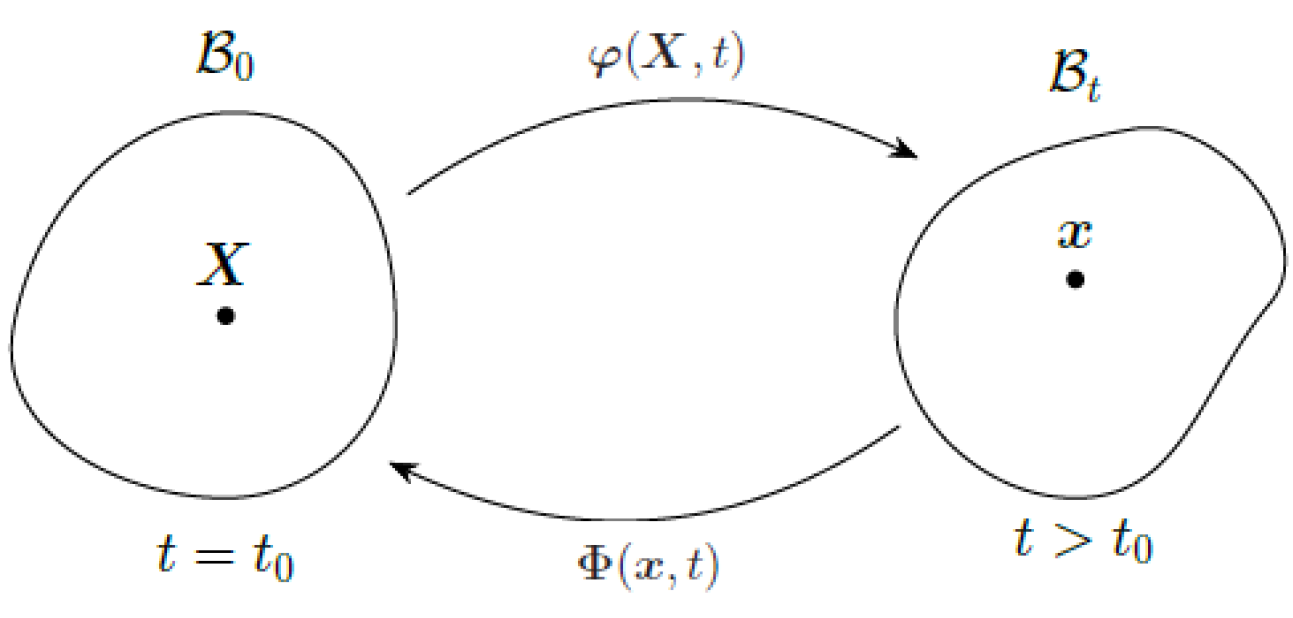
\includegraphics[scale=0.25]{../images/potato.png}
	\caption{Configurations of body in motion}
	\label{fig:potato}
\end{figure}

configurations and motion of a body (figure \ref{fig:potato})

We define a nonlinear deformation map $\varphi$, which describes
the motion of the body. The deformation map has to be unique, continuous
and differentiable and maps the points X in the material configuration
to the places x in the spatial configuration 

\begin{equation}
x=\varphi(X,t)\,with\,\varphi\colon\beta_{0}\rightarrow\beta_{t}
\end{equation}


This description is common in solid mechanics and is denoted as the
Lagrangian description of motion: the motion is characterized with
respect to the material coordinates and one follows the movement of
a particle in time. Inverse mapping is described using 

\begin{equation}
X=\varphi(x,t) , with, \varphi: \beta_{t}\rightarrow\beta_{0}
\end{equation}


Using Lagrangian description displacement field u can be determined
as the difference of spatial and material coordinate system.

\begin{equation}
u(X,t)=x(X,t)-X\label{Lagrangian displacement field}
\end{equation}







\subsubsection{Kinetics \citep{FEM}}

The derivation of the kinetic formulation for FE structure is based
on the above described principle of structural displacement and D\textquoteright Alembert
principle in Lagrangian formulation.

According to D\textquoteright Alembert principle the sum of the virtual
work of all forces acting on the body must be zero. Hence, the sum
of the virtual work of the inertial forces, the internal forces and
the applied external body force over an arbitrary volume $V_{0}$,
and the applied surface force over an infinitesimal area $A_{0}$
of $V_{0}$ equals zero, i.e.


\begin{equation}
-\int_{V_{0}} \delta u^{T}\rho_{0}\textbf{$\ddot{u}$}dV_{0}-\int_{V_{0}}\delta\epsilon^{T}H\varepsilon dV_{0}+\int_{V_{0}}\delta u^{T} b_{0}dV_{0}+\int_{A_{0}}\delta u^{T}p_{0}dA_{0}=0\label{D'Alembert principle}
\end{equation}


let $\rho_{0}$ represent the material density, $b_{0}$ the vector
of the applied external body force over $V_{0}$, $p_{0}$ the vector
of the applied external surface force over $A_{0}$ and the strain
tensor. The term $H$ is the, so called, material matrix defined for
homogeneous, elastic and isotropic materials, with which the material
law is described.

The substitution of Eq.(\ref{Lagrangian displacement field}) into
the first summand of Eq.(\ref{D'Alembert principle}) leads to the
following series of equations: 

\begin{equation}
\int_{V_{0}}\delta u^{T}\rho_{0}\textbf{$\ddot{u}$}dV_{0}\,\,=\delta z_{F}^{T}\sum_{e=1}^{n_{E}}{\sum}\left(T^{e^{T}}\int_{V_{0}^{e}}N^{eT}(x)\rho_{0}^{e}(x)N^{e}(x)dVT^{e}\right)\ddot{z}_{F}
\end{equation}

\begin{equation}
\mathrm{=\delta z_{F}^{T}\sum_{e=1}^{n_{E}}{\sum}{T^{e}}^{T}M^{e}T^{e}\ddot{z}_{F}}
\end{equation}

\begin{equation}
\mathrm{=\delta\boldsymbol{z_{F}^{T}}\boldsymbol{M}_{F}\ddot{\boldsymbol{z}}_{F}}\label{first term of D'Alembert principle}
\end{equation}

where,

\[
\mathrm{\mathbf{M^{e}=\int_{\mathbf{V_{0^{e}}}}N^{eT}}(\mathbf{x})\rho^{e}(\mathbf{x})\mathbf{N^{e}}(\mathbf{x})dV}
\]
represents mass matrix for each element of FE structure.

\[
\mathbf{M_{F}=\sum_{e=1}^{n_{E}}T^{eT}M^{e}T^{e}}
\]
represents mass matrix for entire FE structure.

The substitution of Eq.(\ref{Lagrangian displacement field}) and
linearized strain-displacement relation in the second summand of Eq.(\ref{D'Alembert principle}) leads to the following:


\begin{equation}
\mathrm{\mathrm{\int_{V_{0}}\delta\mathbf{\varepsilon^{T}H\varepsilon}dV_{0}=\delta\mathbf{z}_{F}^{T}\sum_{e=1}^{n_{E}}(\mathbf{T}^{eT}\int_{V_{0^{e}}}\mathbf{B}^{eT}(\mathbf{x})\mathbf{H}^{e}\mathbf{B}^{e}(\mathbf{x})dV\mathbf{T}^{e})\mathbf{z}_{F}}}
\end{equation}


\[
\mathrm{\mathrm{=\delta}\mathbf{z}_{F}^{T}\sum_{e=1}^{n_{E}}\mathbf{T}^{eT}\mathbf{K}^{e}\mathbf{T}^{e}\mathbf{\mathbf{z}}_{F}}
\]
\begin{equation}
\mathrm{\mathrm{=\delta}\mathbf{z}_{F}^{T}\mathbf{K}_{F}\mathbf{z}_{F}}\label{second term of D'Alembert principle}
\end{equation}


where,
\[
\mathrm{\mathbf{K}^{e}=\int_{V_{0}}\mathbf{B}^{eT}(\mathbf{x})\mathbf{H}^{e}\mathbf{B}^{e}(\mathbf{x})dV}
\]
represents linear stiffness matrix for each element of FE structure.

\[
\mathrm{\mathbf{K}_{F}=\sum_{e=1}^{n_{E}}\mathbf{T}^{e}\mathbf{K}^{e}\mathbf{T}^{e}}
\]
represent linear stiffness matrix of whole FE structure.


For the third summand of Eq.(\ref{D'Alembert principle}), the definition
of the body force for each element of the FE structure is used, using
$b_{0}$=Element material density ($\rho$) {*} gravity ($g$)

\begin{equation}
\mathrm{\mathrm{\int_{\mathbf{A_{0}}}\delta\mathbf{u^{T}}\mathbf{b_{0}}dV_{0}=\delta\mathbf{z}_{F}^{T}\sum_{e=1}^{n_{\mathcal{E}}}(T^{eT}\int_{V_{0}^{e}}\mathbf{N^{eT}}(\mathbf{x})\rho_{0}^{e}(\mathbf{x})dV\mathbf{\Gamma^{e}})g}}
\end{equation}
\begin{equation}
\mathrm{\mathrm{=\delta\mathbf{z}_{F}^{T}\sum_{e=1}^{n_{E}}\mathbf{T^{eT}}\mathbf{f}_{g}^{e}=\delta\mathbf{z}_{F}^{T}\mathbf{F_{g}}}}\label{third term of D'Alembert principle}
\end{equation}

where,
\[
f_{g}^{e} = \int_{V_{0}^{e}} N^{eT}(x) \rho_{0}^{e}(x) dV \Gamma^{e}g
\]
represent body force vector for each element.

\[
\mathrm{\mathbf{F}_{g}=\sum_{e=1}^{n_{E}}\mathbf{T^{eT}}\mathbf{f}_{g}^{e}}
\]
represent body force vector for whole FE structure.

Finally, for the last summand of Eq. (\ref{D'Alembert principle})
the utilization of Eq. (\ref{Lagrangian displacement field}) gives

\begin{equation}
\mathrm{\int_{\mathbf{V_{0}}}\delta\mathbf{u^{T}}\mathbf{p_{0}}dA_{0}=\delta\mathbf{z}_{F}^{T}\sum_{e=1}^{n_{\mathcal{E}}}T^{eT}\int_{V_{0}^{e}}\mathbf{N^{eT}}(\mathbf{x})\rho_{0}^{e}(\mathbf{x})dA\mathbf{\Gamma^{e}}}
\end{equation}
\begin{equation}
\mathrm{\mathrm{=\delta\mathbf{z}_{F}^{T}\sum_{e=1}^{n_{E}}\mathbf{T^{eT}}\mathbf{f}_{p}^{e}=\delta\mathbf{z}_{F}^{T}\mathbf{F}_{p}}}\label{fourth term of D'Alembert principle}
\end{equation}


where,
\[
\mathrm{\mathbf{f}_{p}^{e}=\int_{V_{0}^{e}}\mathbf{N^{eT}}(\mathbf{x})\rho_{0}^{e}(\mathbf{x})dA\mathbf{\Gamma^{e}}}
\]
represent external applied on surface of each element.
\[
\mathrm{\mathbf{F}_{p}=\sum_{e=1}^{n_{E}}\mathbf{T^{eT}}\mathbf{f}_{p}^{e}}
\]
represent external force applied on surface of whole FE structure.

Gathering Eq. (\ref{first term of D'Alembert principle}), (\ref{second term of D'Alembert principle}),
(\ref{third term of D'Alembert principle}), and (\ref{fourth term of D'Alembert principle})
and substituting them in Eq. (\ref{D'Alembert principle}) leads to 

\begin{equation}
\delta\mathbf{z}_{F}^{T}(\mathbf{M}_{F}\ddot{\boldsymbol{z}}_{F}+\mathbf{K}_{F}\mathbf{z}_{F}+\mathbf{F_{g}}+\mathbf{F}_{p})=0\label{LTI equation of motion ... undamped}
\end{equation}


which is general second order LTI equation of motion for undamped
FE structure.

If damping effects are to be considered, the definition of the associated
parameter is essential. The simplest, and most commonly used, damping
model assumes the damping to be linearly proportional to the structure\textquoteright s
velocity. This leads to the following equation for linearly damped
FE structures in matrix form 
\begin{equation}
\mathrm{\mathbf{M}_{F}\ddot{\boldsymbol{z}}_{F}+\mathbf{D}_{F}\mathbf{\dot{z}}_{F}+\mathbf{K}_{F}\mathbf{z}_{F}=\mathbf{F}}
\end{equation}


with \textbf{D\textsubscript{\textbf{F}}} being the structural damping
matrix and \textbf{F = F\textsubscript{\textbf{g}}}+\textbf{F\textsubscript{\textbf{p}}}used
for total force acting on structure. The elemental damping can be
formulated in similar pattern as for other matrix described above.

From now on we will drop the suffix F used to represent system matrix
and vectors of FE structure, so equation can be written as 

\begin{equation}
\mathbf{M}\ddot{\mathbf{\boldsymbol{z}}}+\mathbf{D}\mathbf{\dot{z}}+\mathbf{K}\mathbf{z}=\mathbf{F}\label{final equtation of motion FE}
\end{equation}


%\subsection{FEM Tools}



\section{Simulation Setup}
\subsection{Sphere vs Rigid Plane}
In this simulation the collision of two elastic spheres is studied. Both the spheres have the same magnitude of velocity but opposite directions. As newtons third law of motion states "For every action, there is an equal and opposite reaction", to simplify the model and computation, instead of simulation two spheres colliding, a single sphere colliding against a rigid plane can be simulated. This setup would be equivalent to the original problem as both the spheres are the same in all aspects except for having different directions of velocities.

\begin{figure}[H]
	\centering
	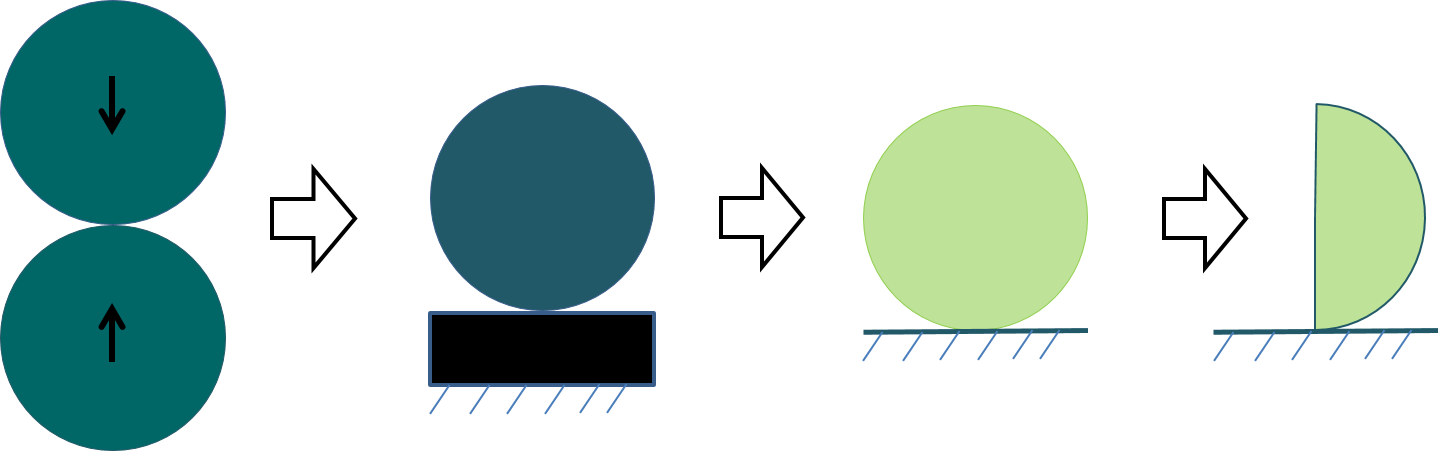
\includegraphics[scale=0.5]{../images/SimulationSetup/sphere2D.png}
\end{figure}
\subsection{Symmetry}
To further simplify the model, instead of considering the complete sphere, only a 2D semi-circular cross-section is considered. As the spheres are symmetric about the central rotational axis and the angle of contact is 90 degrees, there would not be any velocity in the Y direction. 

\subsection{Mesh}

\begin{figure}[H]
    \centering
	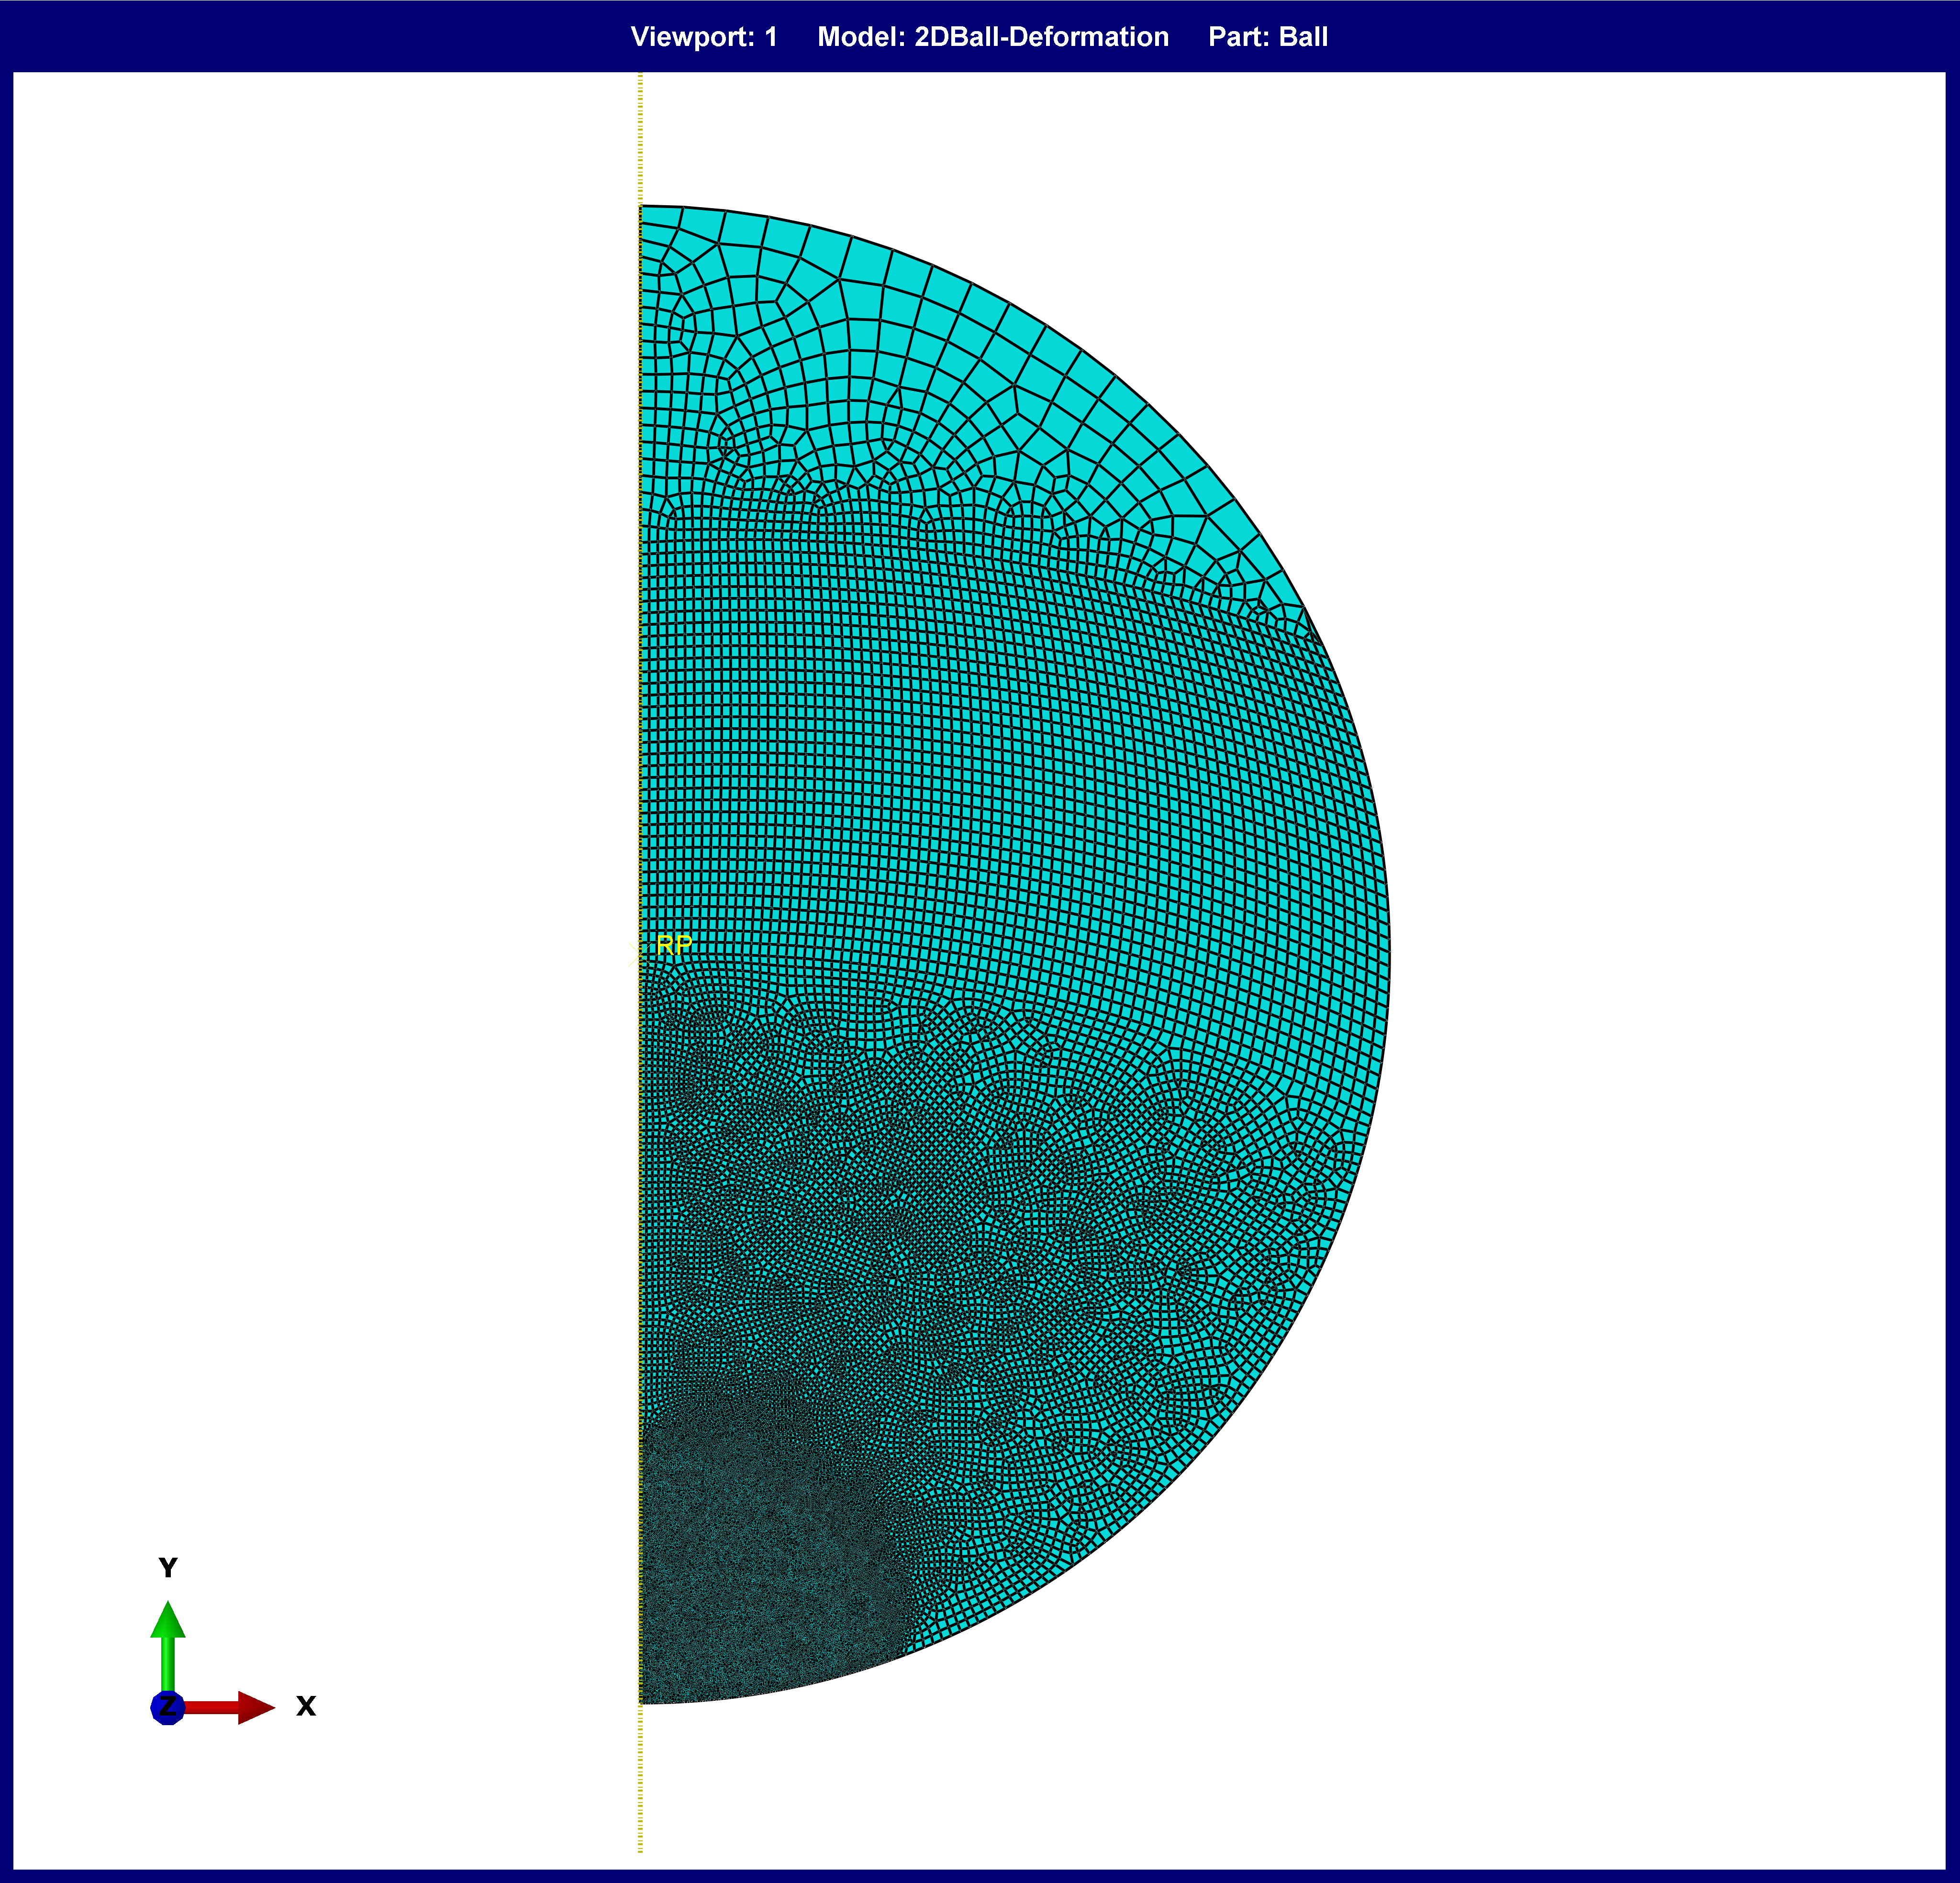
\includegraphics[scale=0.5]{../images/Mesh/Mesh.eps}
	\caption{Mesh}
	\label{fig:mesh}
\end{figure}

To create this setup Abaqus CAE provides an option to create axis-symmetric model. The figure \ref{fig:mesh} shows the mesh used in the simulation. A good mesh for this simulation would have to be finer at the bottom i.e. closer to the surface of contact. To create this mesh, the semicircle was divided into fours sections. The section closer to the surface of contact has a finer mesh and the region away from the contact surface has a course mesh. In figure \ref{fig:mesh} we see the four partitions and the section of the surface of contact has a very fine mesh and the region away from the surface of contact has a course mesh.


\begin{figure}[H]
    \centering
	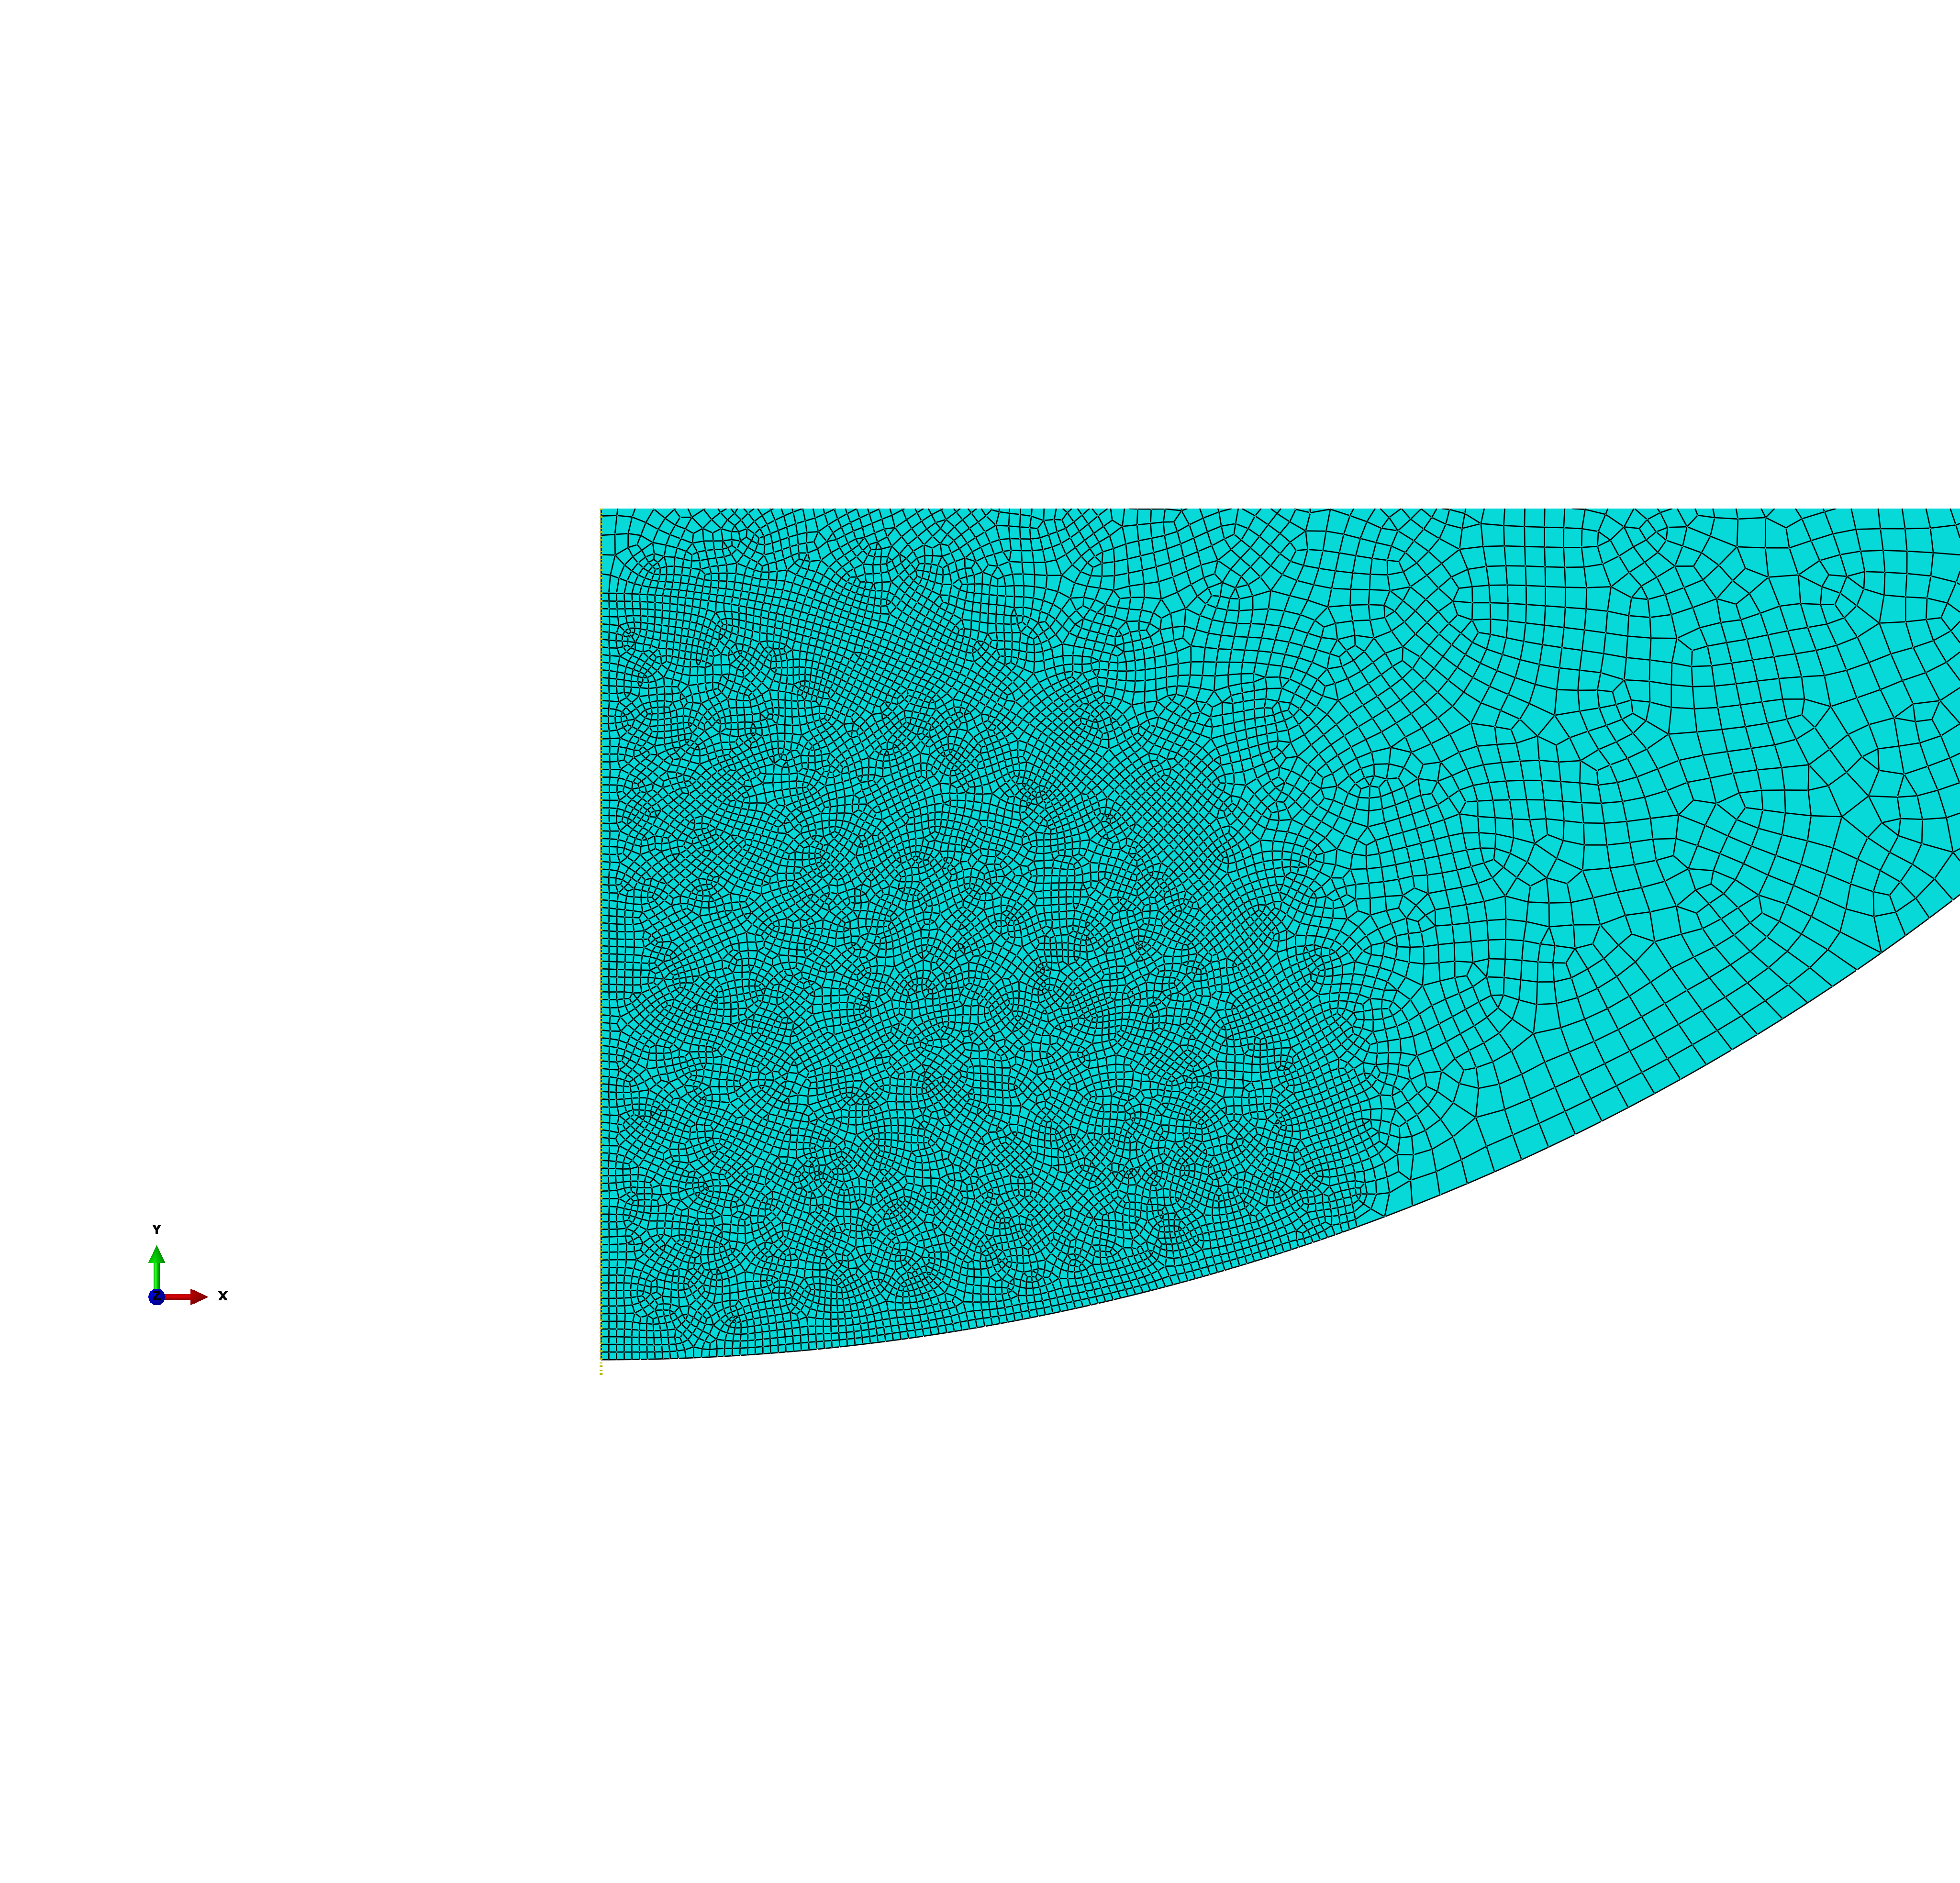
\includegraphics[scale=0.5]{../images/Mesh/Mesh_Bottom.eps}
	\caption{Bottom Half of Mesh}
	\label{fig:mesh_bottom_half}
\end{figure}

The figure \ref{fig:mesh_bottom_half} shows an enlarged image of the bottom half of the mesh. We can see the degree of fineness of the mesh compared to the other half of the sphere.


\subsection{Rigid Plane}

The figure \ref{fig:plane} shows the rigid plane against which the sphere would be colliding. This plane is an axisymmetric, analytical rigid surface. Analytical rigid surfaces are geometric surfaces with profiles that can be described with straight and curved line segments. These profiles can be swept along a generator vector or rotated about an axis to form a three-dimensional surface. An analytical rigid surface does not contribute to the rigid body's mass or inertia properties.

\begin{figure}[H]
    \centering
	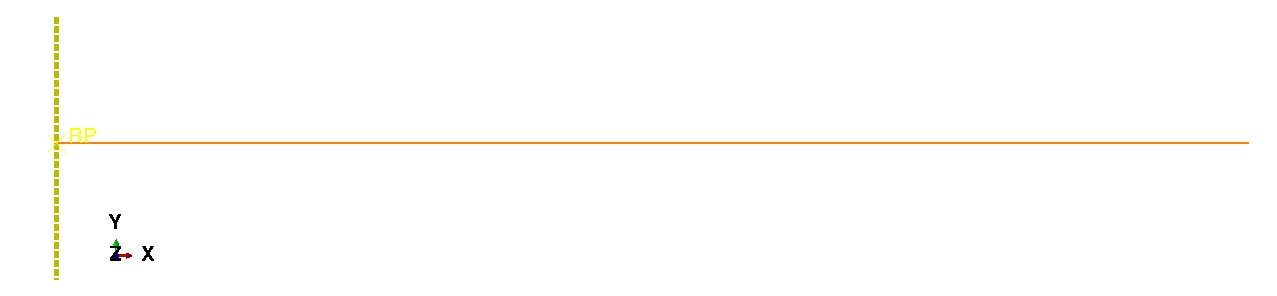
\includegraphics[scale=0.5]{../images/SimulationSetup/Plane.eps}
	\caption{Rigid Plane}
	\label{fig:plane}
\end{figure}


\subsection{Assembly}

The final assembly is of the sphere in contact with the rigid plane as shown in figure \ref{fig:assembly}. The sphere is given a velocity in the $-y$ direction. The starting point of the simulation is when the sphere is in contact with the plane and is about the collide with the plane.
\begin{figure}[H]
    \centering
	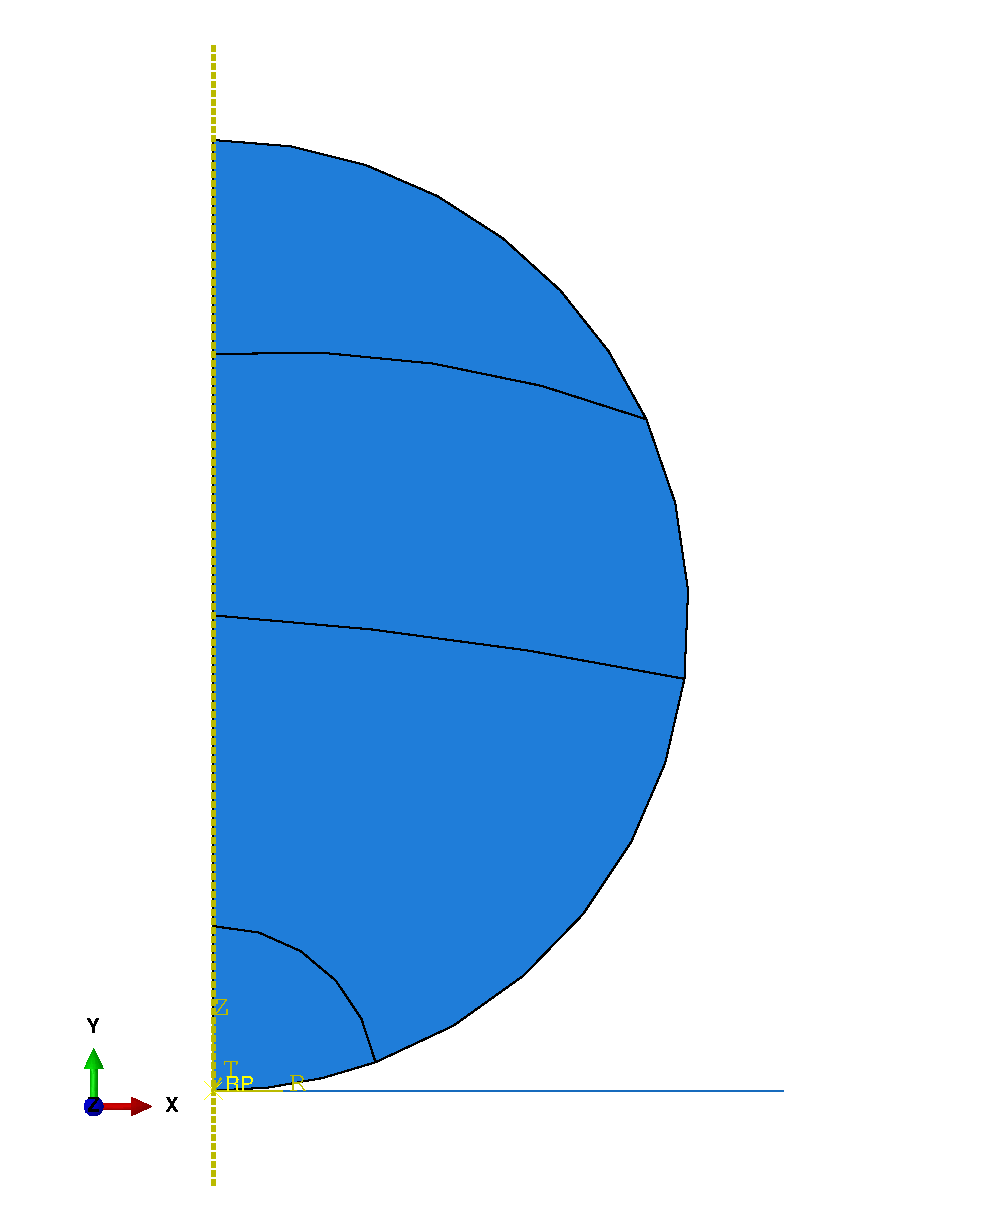
\includegraphics[scale=0.5]{../images/SimulationSetup/Assembly.eps}
	\caption{Assembly}
	\label{fig:assembly}
\end{figure}



\section{Measurement Quantities}

\subsection{Displacement}

\begin{wrapfigure}{R}{0.5\textwidth}
  \begin{center}
	\includegraphics[scale=1]{../images/Mesh/Center.eps}
  \end{center}
  \caption{Center of sphere}
  \label{fig:center}
\end{wrapfigure}

%\begin{figure}[H]
%    \centering
%	\includegraphics[scale=0.5]{../images/Mesh/Center.eps}
%	\caption{Assembly}
%	\label{fig:assembly}
%\end{figure}
To measure the displacement of the body, the displacement of the center of mass was measured. The center of mass of the of a sphere is located at the geometric center of the sphere. The figure \ref{fig:center} shows the center of the 2D semi-circle in red, which was considered as the sphere of the model. To measure the displacement center of mass of the sphere, the displacement of center of the semicircle was considered.

\subsection{Kinetic Energy}

The kinetic energy of an object is the energy that it possesses due to its motion. It is expected that some of the kinetic energy will be converted to strain energy, which can be seen by vibrations in the sphere. The kinetic energy will also be used to calculate the coefficient of restitution of the sphere for various impact velocities.

\begin{equation}
Kinetic Energy(KE) = \frac{mv^{2}}{2}
\end{equation}
 
where $m$ is the mass of the object and $v$ is the velocity of the object.

\subsection{Strain Energy}

The strain energy is the energy stored by a system undergoing deformation. During a collision, a part of the kinetic energy is converted into strain energy. This conversion of kinetic energy to strain energy is ignored due to the quasi static assumptions. This strain energy can also be observed as vibration on the body of the object. When the load is removed,

\begin{equation}
Strain Energy(U) = \frac{V\sigma\epsilon}{2}
\end{equation}

where $V$ is volume, $\sigma$ is stress and $\epsilon$ is strain.

\subsection{Coefficient of Restitution}

The coefficient of restitution is an effective method of understanding the loss of energy in a body during collisions. The coefficient of restitution is a measure of the restitution of kinetic energy after the collision of two objects. 
The coefficient of restitution is calculated by,
\begin{equation}
COR = \frac{-Velocity\, after\, impact}{Velocity\, before\, impact}
\end{equation}
\section{Verification}

To verify the correctness of the simulation setup, various meshes were tried. 
As Abaqus CAE has an option to automatically choose a suitable timestep, the automatic option was chosen.
The validity of considering a a 2D semi circle instead of a complete sphere was check by confirming the mass of the model in the to the calculated mass of the sphere of the same material.